% Options for packages loaded elsewhere
\PassOptionsToPackage{unicode}{hyperref}
\PassOptionsToPackage{hyphens}{url}
\documentclass[
]{article}
\usepackage{xcolor}
\usepackage{amsmath,amssymb}
\setcounter{secnumdepth}{5}
\usepackage{iftex}
\ifPDFTeX
  \usepackage[T1]{fontenc}
  \usepackage[utf8]{inputenc}
  \usepackage{textcomp} % provide euro and other symbols
\else % if luatex or xetex
  \usepackage{unicode-math} % this also loads fontspec
  \defaultfontfeatures{Scale=MatchLowercase}
  \defaultfontfeatures[\rmfamily]{Ligatures=TeX,Scale=1}
\fi
% \usepackage{lmodern}
\ifPDFTeX\else
  % xetex/luatex font selection
\fi
% Use upquote if available, for straight quotes in verbatim environments
\IfFileExists{upquote.sty}{\usepackage{upquote}}{}
\IfFileExists{microtype.sty}{% use microtype if available
  \usepackage[]{microtype}
  \UseMicrotypeSet[protrusion]{basicmath} % disable protrusion for tt fonts
}{}
\makeatletter
\@ifundefined{KOMAClassName}{% if non-KOMA class
  \IfFileExists{parskip.sty}{%
    \usepackage{parskip}
  }{% else
    \setlength{\parindent}{0pt}
    \setlength{\parskip}{6pt plus 2pt minus 1pt}}
}{% if KOMA class
  \KOMAoptions{parskip=half}}
\makeatother
\usepackage{longtable,booktabs,array}
\newcounter{none} % for unnumbered tables
\usepackage{calc} % for calculating minipage widths
% Correct order of tables after \paragraph or \subparagraph
\usepackage{etoolbox}
\makeatletter
\patchcmd\longtable{\par}{\if@noskipsec\mbox{}\fi\par}{}{}
\makeatother
% Allow footnotes in longtable head/foot
\IfFileExists{footnotehyper.sty}{\usepackage{footnotehyper}}{\usepackage{footnote}}
\makesavenoteenv{longtable}
\usepackage{graphicx}
\makeatletter
\newsavebox\pandoc@box
\newcommand*\pandocbounded[1]{% scales image to fit in text height/width
  \sbox\pandoc@box{#1}%
  \Gscale@div\@tempa{\textheight}{\dimexpr\ht\pandoc@box+\dp\pandoc@box\relax}%
  \Gscale@div\@tempb{\linewidth}{\wd\pandoc@box}%
  \ifdim\@tempb\p@<\@tempa\p@\let\@tempa\@tempb\fi% select the smaller of both
  \ifdim\@tempa\p@<\p@\scalebox{\@tempa}{\usebox\pandoc@box}%
  \else\usebox{\pandoc@box}%
  \fi%
}
% Set default figure placement to htbp
\def\fps@figure{htbp}
\makeatother
\setlength{\emergencystretch}{3em} % prevent overfull lines
\providecommand{\tightlist}{%
  \setlength{\itemsep}{0pt}\setlength{\parskip}{0pt}}
\usepackage[]{natbib}
\bibliographystyle{plainnat}
\makeatletter
\@ifpackageloaded{subcaption}{}{\usepackage{subcaption}}
\@ifpackageloaded{caption}{}{\usepackage{caption}}
\captionsetup[subfigure]{margin=0.5em}
\AtBeginDocument{%
\renewcommand*\figurename{Figure}
\renewcommand*\tablename{Table}
}
\AtBeginDocument{%
\renewcommand*\listfigurename{List of Figures}
\renewcommand*\listtablename{List of Tables}
}
\newcounter{pandoccrossref@subfigures@footnote@counter}
\newenvironment{pandoccrossrefsubfigures}{%
\setcounter{pandoccrossref@subfigures@footnote@counter}{0}
\begin{figure}\centering%
\gdef\global@pandoccrossref@subfigures@footnotes{}%
\DeclareRobustCommand{\footnote}[1]{\footnotemark%
\stepcounter{pandoccrossref@subfigures@footnote@counter}%
\ifx\global@pandoccrossref@subfigures@footnotes\empty%
\gdef\global@pandoccrossref@subfigures@footnotes{{##1}}%
\else%
\g@addto@macro\global@pandoccrossref@subfigures@footnotes{, {##1}}%
\fi}}%
{\end{figure}%
\addtocounter{footnote}{-\value{pandoccrossref@subfigures@footnote@counter}}
\@for\f:=\global@pandoccrossref@subfigures@footnotes\do{\stepcounter{footnote}\footnotetext{\f}}%
\gdef\global@pandoccrossref@subfigures@footnotes{}}
\@ifpackageloaded{float}{}{\usepackage{float}}
\floatstyle{ruled}
\@ifundefined{c@chapter}{\newfloat{codelisting}{h}{lop}}{\newfloat{codelisting}{h}{lop}[chapter]}
\floatname{codelisting}{Listing}
\newcommand*\listoflistings{\listof{codelisting}{List of Listings}}
\makeatother
\usepackage{bookmark}
\IfFileExists{xurl.sty}{\usepackage{xurl}}{} % add URL line breaks if available
\urlstyle{same}
% fallback for those not using the hyperref driver hyperxmp:
\makeatletter
\@ifundefined{xmpquote}{\newcommand{\xmpquote}[1]{#1}}{}
\makeatother
\hypersetup{
  colorlinks=true,linkcolor=red,urlcolor=red,citecolor=red,anchorcolor=red,filecolor=red,
  pdfcreator={LaTeX via pandoc}}

\author{}
\date{}

\IfFileExists{seqsplit.sty}{\usepackage{seqsplit}}{\newcommand{\seqsplit}[1]{#1}}
\protected\def\breakseq#1{\seqsplit{#1}}
\protected\def\breaktt#1{\begingroup\ttfamily\seqsplit{#1}\endgroup}
\title{Self-Improvement Agent Harness: A Deterministic SIA Exemplar}
\author{Daniel Ari Friedman\\\footnotesize{Active Inference Institute}\\\footnotesize{\texttt{daniel@activeinference.institute}}\\\footnotesize{\href{https://orcid.org/0000-0001-6232-9096}{ORCID: 0000-0001-6232-9096}} \\ \footnotesize{DOI: \href{https://doi.org/10.5281/zenodo.20453879}{10.5281/zenodo.20453879}}}
\date{\today}

\usepackage[margin=0.75in]{geometry}
\usepackage{graphicx}

\begin{document}

\begin{titlepage}
\centering
\vspace*{2cm}
{\LARGE\bfseries Self-Improvement Agent Harness: A Deterministic SIA Exemplar\par}
\vspace{0.75em}
{\large Meta → Target → Feedback loops with public/private task splits\par}
\vfill
\makeatletter
{\@author\par}
\vspace{1em}
{\@date\par}
\makeatother
\vfill
\end{titlepage}
\thispagestyle{empty}
\tableofcontents
\newpage


\section{Abstract}\label{sec:abstract}

This exemplar documents \textbf{template\_sia}, a deterministic
implementation of the Self-Improvement Agent (SIA) harness contract
described in \citep{sia2026}. The default pipeline replays
fixture-backed generations for the \texttt{mini\_classify} task; opt-in
live mode runs bounded target subprocesses and optional Ollama-backed
meta/feedback steps.

\textbf{Run snapshot.} Task \texttt{mini\_classify}, run 1, 3
generation(s), live=false. Final accuracy=0.8333 over 6 held-out
samples. Values are injected by
\breaktt{scripts/z\_generate\_manuscript\_variables.py} after analysis.

\textbf{Keywords:} self-improvement agents, benchmark harness,
reproducible evaluation, agent loops

\newpage

\section{Introduction}\label{sec:introduction}

This exemplar ships \textbf{template\_sia}, a deterministic research
harness for Self-Improvement Agent (SIA) loops \citep{sia2026}. It
documents how the template repository separates generic orchestration
(\breaktt{infrastructure/sia/}) from a reproducible project surface
(\breaktt{projects/templates/template\_sia/}) without vendoring the
upstream \href{https://github.com/hexo-ai/sia}{upstream SIA orchestrator
repository}.

Compared with the AutoResearch exemplar, SIA focuses on \textbf{meta \texorpdfstring{\ensuremath{\to}}{->}
target \texorpdfstring{\ensuremath{\to}}{->} feedback} generations with public/private task splits rather
than candidate-model search and readiness gates. Default CI replays
fixture-backed generations; live mode remains opt-in.

\textbf{Scope.} The bundled \texttt{mini\_classify} task is a threshold
classifier on one feature column. Results demonstrate harness wiring and
artifact contracts---not state-of-the-art accuracy.

\textbf{Run contract.} Task \texttt{mini\_classify}, run 1, up to 3
generation(s), live=false.

\newpage

\section{Methodology}\label{sec:methodology}

\subsection{SIA loop}\label{sia-loop}

The harness implements a three-agent cycle:

\begin{enumerate}
\def\labelenumi{\arabic{enumi}.}
\tightlist
\item
  \textbf{Meta} --- proposes or seeds a target agent for generation
  \(n\).
\item
  \textbf{Target} --- runs against public task data and writes
  \breaktt{agent\_execution.json}.
\item
  \textbf{Feedback} --- reads private evaluation metrics and proposes
  improvements for generation \(n+1\).
\end{enumerate}

\begin{figure}
\centering
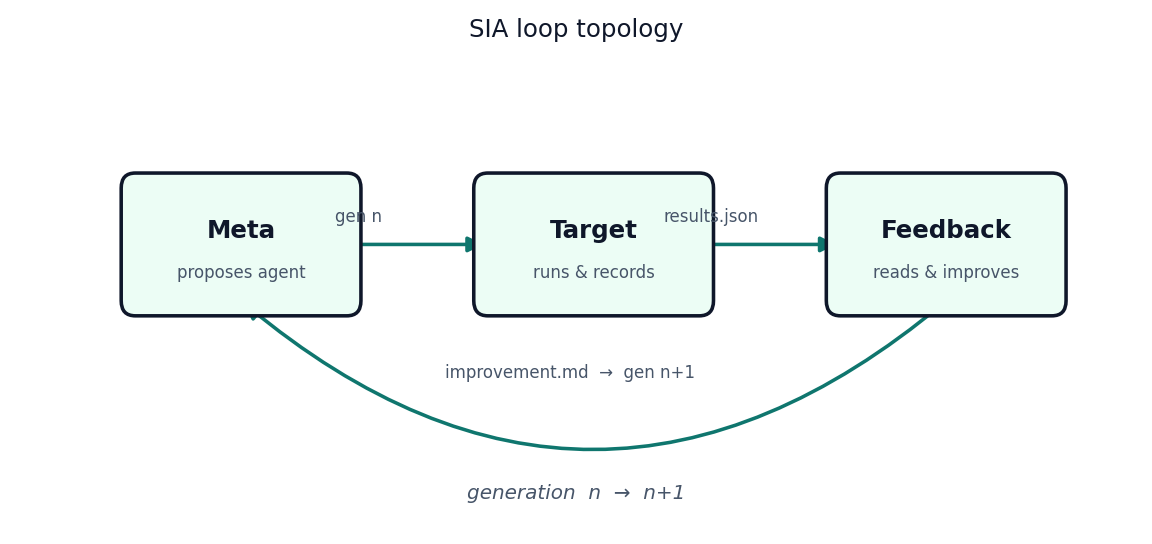
\includegraphics[width=0.9\linewidth,height=0.50\textheight,keepaspectratio,alt={Meta \texorpdfstring{\ensuremath{\to}}{->} Target \texorpdfstring{\ensuremath{\to}}{->} Feedback loop topology for the SIA harness, generated programmatically by write\_sia\_loop\_topology.}]{../figures/sia_loop_topology.png}
\caption{Meta \texorpdfstring{\ensuremath{\to}}{->} Target \texorpdfstring{\ensuremath{\to}}{->} Feedback loop topology for the SIA harness,
generated programmatically by
\protect\breaktt{write\_sia\_loop\_topology}.}\label{fig:sia-loop-topology}
\end{figure}

Artifacts land under \texttt{output/runs/run\_\{id\}/gen\_\{n\}/} with
\texttt{target\_agent.py}, \breaktt{agent\_execution.json}, optional
\texttt{improvement.md}, and canonical \texttt{results.json}.

\subsection{Task layout}\label{task-layout}

Each task exposes:

\begin{itemize}
\tightlist
\item
  \texttt{data/public/} --- agent-visible instructions and data
  (\texttt{task.md}, \texttt{train.csv}, \texttt{evaluate.py}).
\item
  \texttt{data/private/} --- held-out labels for evaluation only.
\item
  \breaktt{reference/reference\_target\_agent.py} --- deterministic
  baseline.
\end{itemize}

The exemplar task \texttt{mini\_classify} is a threshold classifier on a
single feature column.

\subsection{Determinism contract}\label{determinism-contract}

When \breaktt{sia.live:\ false} (default), generations replay recorded
fixtures from \breaktt{src/fixtures/recorded\_generations/}. CI never
executes generated agent code or calls external LLM APIs.

Pass \texttt{-\/-live-sia} to \breaktt{scripts/run\_sia\_loop.py} for
bounded subprocess execution and optional Ollama feedback when a model
is configured.

\subsection{Per-generation metric
overview}\label{per-generation-metric-overview}

The heatmap below provides a compact overview of per-generation accuracy
and sample count, enabling at-a-glance comparison across runs.

\begin{figure}
\centering
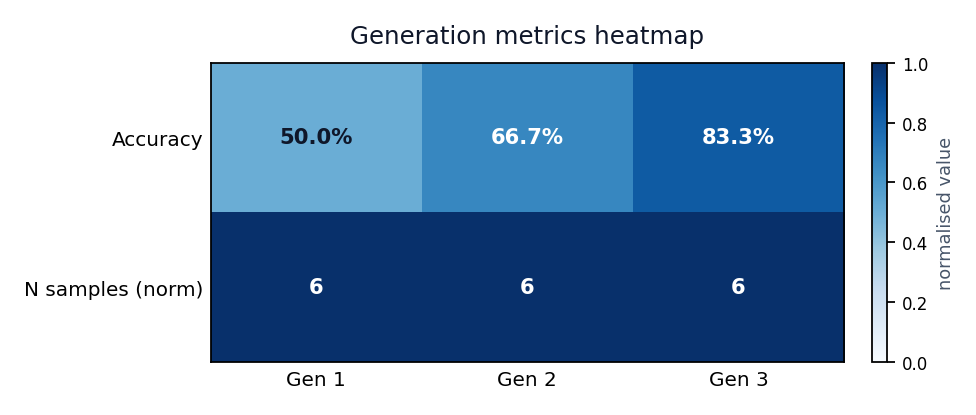
\includegraphics[width=0.8\linewidth,height=0.50\textheight,keepaspectratio,alt={Per-generation metric heatmap showing accuracy and sample count across SIA generations.}]{../figures/sia_generation_heatmap.png}
\caption{Per-generation metric heatmap showing accuracy and sample count
across SIA generations.}\label{fig:sia-generation-heatmap}
\end{figure}

\newpage

\section{Results}\label{sec:results}

tbl.~\ref{tbl:sia-metrics} summarizes fixture-replay metrics for the
bundled run.

\begin{longtable}[]{@{}llrr@{}}
\caption{SIA generation metrics (fixture
replay).}\label{tbl:sia-metrics}\tabularnewline
\toprule\noalign{}
Gen & Metric & Value & N \\
\midrule\noalign{}
\endfirsthead
\toprule\noalign{}
Gen & Metric & Value & N \\
\midrule\noalign{}
\endhead
\bottomrule\noalign{}
\endlastfoot
1 & accuracy & 0.5000 & 6 \\
2 & accuracy & 0.6667 & 6 \\
3 & accuracy & 0.8333 & 6 \\
\end{longtable}

Metric delta (final \texorpdfstring{\ensuremath{-}}{-} first generation): 0.3333.

Final injected token: accuracy=0.8333 (n=6).

\begin{figure}
\centering
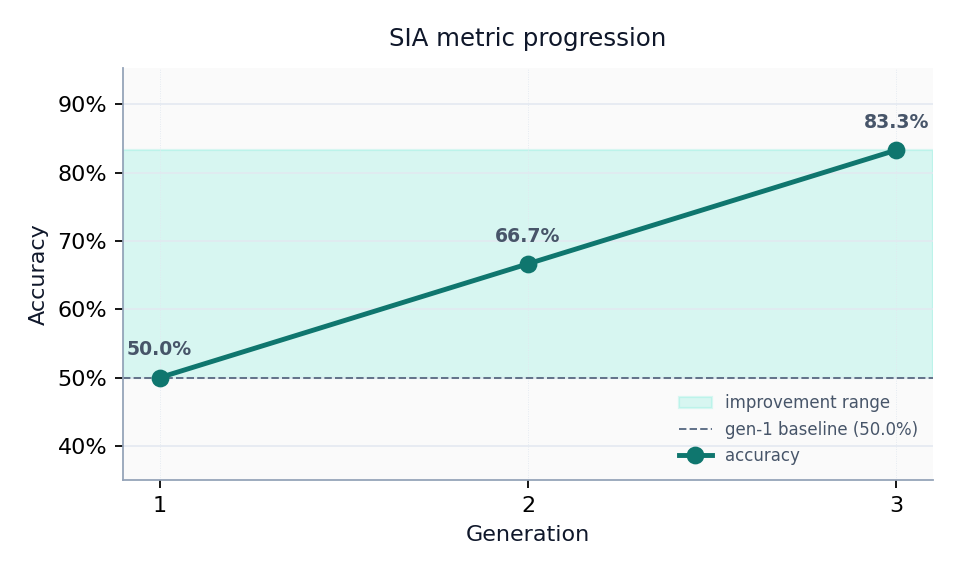
\includegraphics[width=0.85\linewidth,height=0.50\textheight,keepaspectratio,alt={SIA metric progression across generations.}]{../figures/sia_metric_progression.png}
\caption{SIA metric progression across
generations.}\label{fig:sia-metric-progression}
\end{figure}

\subsection{Incremental improvement}\label{incremental-improvement}

The generation-over-generation accuracy delta quantifies the
self-refinement signal at each step of the loop.

\begin{figure}
\centering
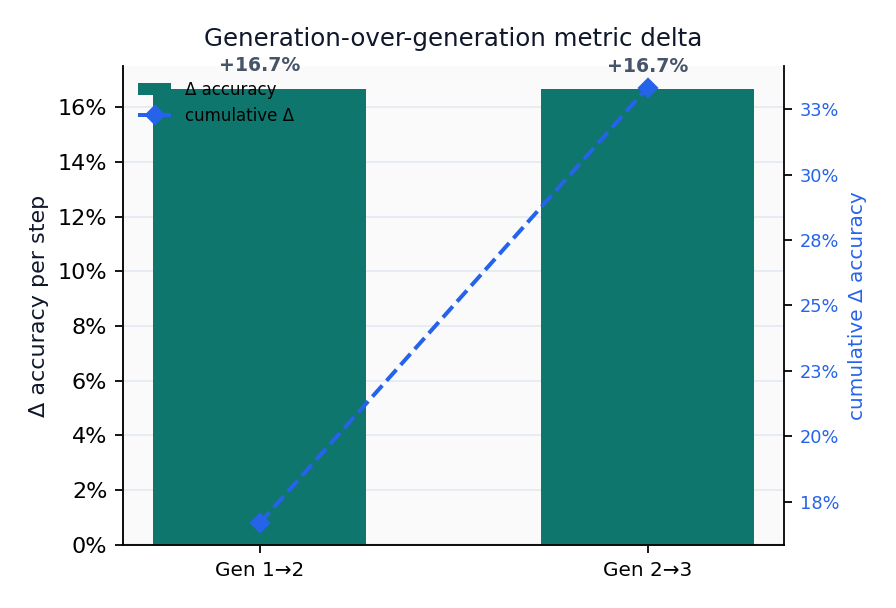
\includegraphics[width=0.8\linewidth,height=0.50\textheight,keepaspectratio,alt={Generation-over-generation metric delta (\texorpdfstring{\ensuremath{\Delta}}{Delta}accuracy) for the SIA loop, illustrating the incremental improvement at each self-refinement step.}]{../figures/sia_improvement_delta.png}
\caption{Generation-over-generation metric delta (\texorpdfstring{\ensuremath{\Delta}}{Delta}accuracy) for the SIA
loop, illustrating the incremental improvement at each self-refinement
step.}\label{fig:sia-improvement-delta}
\end{figure}

\newpage

\section{Conclusion}\label{sec:conclusion}

template\_sia demonstrates how to embed the SIA harness contract in the
Research Project Template without vendoring upstream orchestration code.
Layer 1 (\breaktt{infrastructure/sia/}) owns task validation, evaluation,
context logging, and the generation state machine; Layer 2 wires a
minimal classification task, fixture replay, and manuscript tokens.

\textbf{Non-claims.} This tree is a harness and documentation exemplar.
Fixture-replay metrics (final accuracy=0.8333) validate wiring
only---they are not evidence of state-of-the-art self-improvement. Live
self-modification and external LLM calls remain opt-in; default CI never
executes generated agent code or claims benchmark parity with
\citep{sia2026}.

\newpage

\section{References}\label{sec:references}

See \texttt{references.bib} for BibTeX entries cited in this manuscript,
including \citep{sia2026} and the template repository DOI from
\breaktt{manuscript/config.yaml}.



\clearpage

\bibliography{references}
\end{document}
